\section*{X.  Matrix Derivatives}
        
    In general, we want to be able to combine the powers of matrices and calculus:
    
    \begin{itemize}
        \item \textbf{Matrices}: the ability to store lots of \textbf{data}, and do fast linear operations on all that data at the \textbf{same time}.
        
        \miniex Consider
        
        \begin{equation}
            \blu{w}^T\red{x} =
            \begin{bmatrix}
                \blu{w_1} & \blu{w_2} & \cdots & \blu{w_m}
            \end{bmatrix}
            \begin{bmatrix}
                \red{x_1} \\ \red{x_2} \\ \vdots \\ \red{x_m}
            \end{bmatrix}
            =
            \sum_{i=1}^m \red{x_i}\blu{w_i}
        \end{equation}
        
        In this case, we're able to do $m$ different \textbf{multiplications} at the same time! This is what we like about matrices.
            \note{In this case, we're thinking about vectors as $(m  \times 1)$ matrices.}
        
        \item \textbf{Calculus}: analyzing the way different variables are \textbf{related}: how does changing $x$ affect $y$?
        
        \miniex Suppose we have 
        
        \begin{equation}
            \pderiv{f}{x_1}=10 \qquad 
            \pderiv{f}{x_2}=-5
        \end{equation}
        
        Now we know that, if we increase $x_1$, we increase $f$. This \textbf{understanding} of variables is what we like about derivatives.\\
    \end{itemize}
    
    \begin{concept}
        \vocab{Matrix derivatives} allow us to find \purp{relationships} between large volumes of \gren{data}.
        
        \begin{itemize}
            \item These "relationships" are \vocab{derivatives}: consider $\derivslash{y}{x}$. How does $y$ change if we modify $x$? Currently, we only have \purp{scalar derivatives}.
            
            \item This "data" is stored as \vocab{matrices}: blocks of data, that we can do linear operations (matrix multiplication) on.
        \end{itemize}
        
        Our goal is to work with many scalar derivatives at the \gren{same time}. 
        
        In order to do that, we can apply some \gren{derivative} rules, but we have to do it in a way that \purp{agrees} with \gren{matrix} math.
    \end{concept}
    
    Our work is a careful balancing act between getting the \textbf{derivatives} we want, without violating the \textbf{rules} of matrices (and losing what makes them useful!)
    
    \miniex When we multiply two matrices, their inner shape has to match: in the below case, they need to share a dimension $b$.
    
    \begin{equation}
        \overbrace{
            X
        }^{ (a \times \red{b}) }
        \overbrace{
            Y
        }^{(\red{b} \times c)}
    \end{equation}
    
    We can't do anything that would \textbf{violate} this rule: otherwise, our \textbf{equations} don't make sense, and we get stuck. This means we need to build our math carefully.
    
    First, we'll look at the \textbf{properties} of derivatives. Then figure out how to usefully apply them to \textbf{vectors}, and then \textbf{matrices}.
    
    \secdiv
    
    \subsection*{X.1 \quad Review: Partial Derivatives}
    
        One more comment, though - we may have many different variables floating around. This means we \textbf{have} to use the multivariable \textbf{partial derivative}.\\
        
        \begin{definition}
            The \vocab{partial derivative} 
            
            \begin{equation*}
                \pderiv{B}{A}
            \end{equation*}
            
            Is used when there may be \purp{multiple variables} in our functions.
            
            The rule of the partial derivative is that we keep every \gren{independent} variable other than $A$ and $B$ \purp{fixed}.
        \end{definition}
        
        \miniex Consider $f(x,y) = 2x^2y$.
        
        \begin{equation}
            \pderiv{f}{x} = 2(2x)y
        \end{equation}
        
        Here, we kept $y$ \textit{fixed} - we treat it as if it were an unchanging \textbf{constant}. 
        
        Using the partial derivative lets us keep our work tidy: if \textbf{many} variables were allowed to \textbf{change} at the same time, it could get very confusing. 
            \note{Imagine keeping track of $k$ different variables $x_i$ with $k$ different changes $\Delta x_i$ at the same time! That's a headache.}
        
        If this is too complicated, we can change those variables \textit{one at a time}. We get a partial derivative for each of them, holding the others \textbf{constant}.
        
        Our \textbf{total} derivative is the result of all of those different variables, \textbf{added} together. This is how we get the \textbf{multi-variable chain rule}.\\ 
        
        \begin{definition}
            The \vocab{multi-variable chain rule} in 3-D ($\{x,y,z\}$) is given as
            
            \begin{equation*}
                \deriv{\red{f}}{\blu{s}} 
                = 
                \overbrace{
                    \pderiv{\red{f}}{\pur{x}}
                    \pderiv{\pur{x}}{\blu{s}}
                }^{\text{only modify $x$}}
                +
                \overbrace{
                    \pderiv{\red{f}}{\pur{y}}
                    \pderiv{\pur{y}}{\blu{s}}
                }^{\text{only modify $y$}}
                +
                \overbrace{
                    \pderiv{\red{f}}{\pur{z}}
                    \pderiv{\pur{z}}{\blu{s}}
                }^{\text{only modify $z$}}
            \end{equation*}
            
            If we have $k$ variables $\{x_1,x_2,\dots x_k\}$ we can generalize this as:
            
            \begin{equation*}
                \deriv{\red{f}}   {\blu{s}} = 
                \sum_{i=1}^{k}
                \overbrace{
                    \pderiv{\red{f}}   {\pur{x_i}}
                    \pderiv{\pur{x_i}} {\blu{s}}
                }^{\text{$x_i$ component}}
            \end{equation*}
            
        \end{definition}
    
    \secdiv
    
    \subsection*{X.2 \quad Thinking about derivatives}
    
        The typical definition of derivatives
        
        \begin{equation}
            \lim_{h \rightarrow 0} \frac{f(x+h)-f(x)}{h}
        \end{equation}
        
        Gives an \textit{idea} of what sort of things we're looking for. It reminds us of one piece of information we need:
        
        \begin{itemize}
            \item Our derivative \textbf{depends} on the \textbf{current position} $x$ we are taking the derivative at.
        \end{itemize}
        
        We need this because derivative are \textbf{local}: the relationship between our variables might change if we move to a different \textbf{position}.
        
        But, the problem with vectors is that each component can act \textbf{separately}: if we have a vector, we can change in many different "directions".
        
        \begin{equation}
            A = 
            \begin{bmatrix}
                a_1 \\ a_2 \\ a_3
            \end{bmatrix}
            \qquad
            B = 
            \begin{bmatrix}
                b_1 \\ b_2
            \end{bmatrix}
        \end{equation}
        
        \miniex Suppose we want a derivative $\pderivslash{B}{A}$: $\Delta a_1, \Delta a_2,$ and $\Delta a_3$ could each, separately, have an effect on $\Delta b_1$ and/or $\Delta b_2$. That requires 6 different derivatives, $\pderivslash{b_i}{a_j}$.
            \note{3 dimensions of $A$ times 2 dimensions of $B$: 6 combinations.}
        
        Every component of the input $A$ can potentially modify \textbf{every} component of the output $B$. 
        
        One solution we could try is to just collect all of these derivatives into a \textbf{vector} or \textbf{matrix}.\\
        
        \begin{concept}
            For the \vocab{derivative} between two objects (scalars, vectors, matrices) $\red{A}$ and $\blu{B}$
            
            \begin{equation*}
                \pderiv{\blu{B}}{\red{A}}
            \end{equation*}
            
            We need to get the \purp{derivatives}
            
            \begin{equation*}
                \pderiv{\blu{b_j}}{\red{a_i}}
            \end{equation*}
            
            between every \purp{pair} of elements $\red{a_i}$, $\blu{b_j}$: each pair of elements could have a \gren{relationship}.
            
            The total number of elements (or "size") is...
            
            \begin{equation*}
                \text{Size}\Bigg(  \pderiv{\blu{B}}{\red{A}}  \Bigg) 
                = 
                \text{Size}(\blu{B})
                *
                \text{Size}(\red{A})
            \end{equation*}
            
            Collecting these values into a \gren{matrix} will gives us all the information we need.
        \end{concept}
        
        But, how do we gather them? What should the \textbf{shape} look like? Should we \textbf{transpose} our matrix or not?
    
    \secdiv
    
    \subsection*{X.3 \quad Derivatives: Approximation}
        
        To answer this, we need to ask ourselves \textit{why} we care about these derivatives: their \textbf{structure} will be based on what we need them for.
        
        \begin{itemize}
            \item We care about the \textbf{direction of greatest decrease}, the gradient. For example, we might want to adjust weight vector $w$ to reduce $\loss$.
            
            \item We also want other derivatives that have the \textbf{same} behavior, so we can combine them using the \textbf{chain rule}.
        \end{itemize}
        
        Let's focus on the first point: we want to \textbf{minimize} $\loss$. Our focus is the \textbf{change} in $\loss$, $\Delta \loss$.
            \note{We want to take steps that reduce our loss $\loss$.}
        
        \begin{equation}
            \pderiv{\loss}{w} 
            \approx 
            \frac{\text{Change in }\loss }{ \text{Change in w} }
            =
            \frac{\Delta \loss}{ \Delta w}
        \end{equation}
        
        Thus, we \textbf{solve} for $\Delta \loss$:
            \note{All we do is multiply both sides by $\Delta w$.}
        
        \begin{equation}
            \Delta \loss
            \approx
            \pderiv{\loss}{w} 
            \Delta w
        \end{equation}
        
        Since this derivation was gotten using scalars, we might need a \textbf{different} type of multiplication for our \textbf{vector} and \textbf{matrix} derivatives.\\
        
        \begin{concept}
            We can use derivatives to \vocab{approximate} the change in our output based on our input:
            
            \begin{equation*}
                \Delta \loss
                \approx
                \pderiv{\loss}{\pur{w}} 
                \star
                \Delta \pur{w}
            \end{equation*}
            
            Where the $\star$ symbol represents some type of \purp{multiplication}.
            
        \end{concept}
        
        We can think of this as a \textbf{function} that takes in change in $\Delta w$, and returns an \textbf{approximation} of the loss.
        
        We already understand \textbf{scalar} derivatives, so let's move on to the \textbf{gradient}.
        
    \secdiv
    
    \subsection*{X.4 \quad The Gradient: a vector input, scalar output}
    
        Our plan is to look at every derivative combination of scalars, vectors, and matrices we can.
        
        First, we consider:
        
        \begin{equation}
            \pderiv{ \text{(Scalar) } } { \text{(Vector)} }
            =
            \pderiv{\red{s}}{ \pur{v} } 
        \end{equation}
        
        We'll take $\red{s}$ to be our scalar, and $\pur{v}$ to be our vector. So, our input is a \textbf{vector}, and our output is a \textbf{scalar}.
        
        \begin{equation}
            \Delta \pur{v}
            \longrightarrow
            \boxed{f}
            \longrightarrow
            \Delta \red{s}
        \end{equation}
        
        How do we make sense of this? Well, let's write $\Delta \pur{v}_i$ explicitly:
        
        \begin{equation}
            \overbrace{
                \begin{bmatrix}
                    \Delta \pur{v_1}\\ \Delta \pur{v_2}\\ \vdots \\ \Delta \pur{v_m}
                \end{bmatrix}
            }^{\Delta v}
            \longrightarrow 
            \Delta \red{s}
        \end{equation}
        
        We can see that we have $m$ different \textbf{inputs} we can change in order to change our \textbf{one} output.
        
        So, our derivative needs to have $m$ different \textbf{elements}: one for each element $\pur{v}_i$.
    
    \secdiv
       
    \subsection*{X.5 \quad Finding the scalar/vector derivative}
        
        But how do we shape our matrix? Let's look at our \textbf{rule}.
        
        \begin{equation}
            \Delta \red{s}
            \approx
            \pderiv{\red{s}}{ \pur{v} }  
            \star
            \Delta \pur{v}
                \qquad
                \text{or}
                \qquad
            \Delta \red{s}
            \approx
            \pderiv{\red{s}}{ \pur{v} } 
            \star
            \overbrace{
                \begin{bmatrix}
                    \Delta \pur{v_1}\\ \Delta \pur{v_2}\\ \vdots \\ \Delta \pur{v_m}
                \end{bmatrix}
            }^{\Delta v}
        \end{equation}
        
        How do we get $\Delta \red{s}$? We have so many variables. Let's focus on them one at a time: breaking $\Delta \pur{v}$ into $\Delta \pur{v_i}$, so we'll try to consider each $\pur{v_i}$ \textbf{separately}.
            \note{It's usually possible to change each $\pur{v_i}$, so we have to look at every one of them.}
        
        One problem, though: how can we treat each \textbf{derivative} separately? Each $\Delta \pur{v_i}$ will move our position, which can change a different derivative $\pur{v_k}$: they can \textbf{affect} each other.
    
    \secdiv
    
    \subsection*{X.6 \quad Review: Planar Approximation}
        
        We'll resolve this the same way we did in chapter 3, \textbf{gradient} descent: by taking advantage of the "planar approximation".
        
        The solution is this: assume your function is \textbf{smooth}. The \textbf{smaller} a step you take, the \textbf{less} your derivative has a chance to change.
            \note{This isn't true for big steps, but eventually, if your step is small enough, then the derivative will barely change.}
        
        \miniex Take $f(x)=x^2$. 
        
        \begin{itemize}
            \item If we go from $x=1\rightarrow2$, then our derivative goes from $f'(x)=2 \rightarrow 4$.
            
            \item Let's \textbf{shrink} our step. We go from $x=1\rightarrow1.01$, our derivative goes from $f'(x)=2 \rightarrow 2.02$.
                \begin{itemize}
                    \item Our derivative is almost the same!
                \end{itemize}
        \end{itemize}
        
        if we take a small enough step $\Delta v_i$, then, if our function is \textbf{smooth}, then the derivative will hardly change!
            \note{You could imagine repeatedly shrinking the size of our step, until the change in the derivatives is basically unnoticeable.}
            
        So, if we zoom in enough (shrink the scale of change), then we can \textbf{pretend} the derivative is \textbf{constant}.\\
        
        \begin{concept}
            If you have a \gren{smooth function}, then...
            
            If you take sufficiently \vocab{small steps}, then you can treat the derivatives as \purp{constant}.
        \end{concept}
        
        \phantom{}\\
        
        \begin{clarification*}
            This section is \vocab{optional}.
            
            We can describe "sufficiently small steps" in a more mathematical way:
            
            Our goal is for $\org{f'(x)}$ to be \purp{basically constant}: it doesn't change much. $\Delta \org{f'(x)}$ is \gren{small}. 
            
            Let's say it can't change more then $\pur{\delta}$. 
            
            If you want 
            \begin{itemize}
                \item $\Delta \org{f'(x)}$ to be very small ($|\Delta \org{f'(x)}| < \pur{\delta}$)
                \item It has been proven that...
                \begin{itemize}
                    \item can take a small enough step $|\Delta \red{x}| < \pur{\epsilon}$, and to get that result.
                \end{itemize}
            \end{itemize}
        \end{clarification*}
        
        One way to describe this is to say that our function is (locally) \textbf{flat}: it looks like some kind of plane/hyperplane.
            \note{The word "locally" represents the small step size: we stay in the "local area".}\\
        
        \begin{clarification}
            Why is this \purp{true}? Because a \vocab{hyperplane} can be represented using our \vocab{linear} function 
            
            \begin{equation*}
                f(x) 
                \approx
                \red{\theta^T}x+\theta_0
                =
                \theta_0 + \red{\theta_1}x_1+\red{\theta_2}x_2+\dots+ \red{\theta_m}x_m
            \end{equation*}
            
            If we take a derivative:
            
            \begin{equation*}
                \pderiv{f}{x_i}
                =
                \theta_i
            \end{equation*}
            
            That derivative is a \purp{constant}! It's doesn't change based on \gren{position}.
        \end{clarification}
        
        \begin{figure}[H]
            \centering
                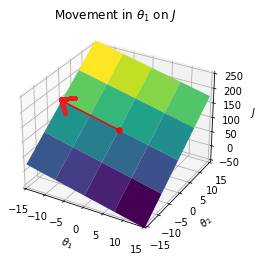
\includegraphics[width=70mm,scale=0.5]{images/gradient_descent_images/theta1_movement_plane.png}
            \caption*{If we take very small steps, we can approximate our function as \textbf{flat}.}
        \end{figure}
        
        
        Why does this help? If our derivative doesn't \textbf{change}, we can combine multiple steps  You can take multiple steps $\Delta \pur{v_i}$ and the order doesn't matter.
            \note{So, you can combine your steps or separate them easily.}
            
        \begin{figure}[H]
            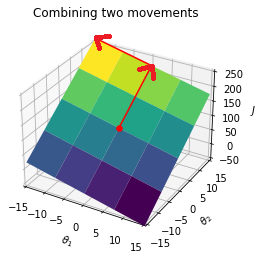
\includegraphics[width=70mm,scale=0.5]{images/gradient_descent_images/thetaboth_movement_plane.png}
            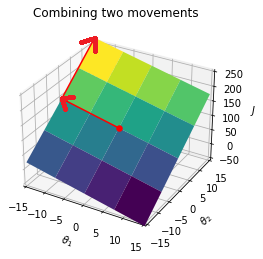
\includegraphics[width=70mm,scale=0.5]{images/gradient_descent_images/thetaboth_movement_plane_reversed.png}
                
            \caption*{We can break up our big step into two smaller steps that are truly independent: order doesn't matter.}
        \end{figure}
        
        
        
        With that, we can add up all of our changes:
        
        \begin{equation}
            \Delta s = 
            \Delta s_{\text{from } v_1}
            +
            \Delta s_{\text{from } v_2}
            +
            \dots
            +
            \Delta s_{\text{from } v_m}
        \end{equation}
    
    \secdiv
    
    \subsection*{X.7 \quad Our scalar/vector derivative}
        
        From this, we can get an \textbf{approximated} version of the MV chain rule.\\
        
        \begin{definition}
            The \purp{multivariable chain rule} \vocab{approximation} looks similar to the multivariable chain rule, but for finite changes $\Delta x_i$.
            
            In 3-D, we get
            
            \begin{equation*}
                \Delta \red{f} 
                = 
                \overbrace{
                    \pderiv{\red{f}}{\pur{x}}
                    \Delta \pur{x}
                }^{\text{$x$ component}}
                +
                \overbrace{
                    \pderiv{\red{f}}{\pur{y}}
                    \Delta \pur{y}
                }^{\text{$y$ component}}
                +
                \overbrace{
                    \pderiv{\red{f}}{\pur{z}}
                    \Delta \pur{z}
                }^{\text{$z$ component}}
            \end{equation*}
            
            In general, we have
            
            \begin{equation*}
                \Delta \red{f} 
                \quad
                = 
                \quad
                \sum_{i=1}^{m}
                \overbrace{
                    \pderiv{\red{f}}   {\pur{x_i}}
                    \Delta \pur{x_i}
                }^{\text{$x_i$ component}}
            \end{equation*}
        \end{definition}
        
        This function lets us add up the effect each component has on our output, using \textbf{derivatives}.
        
        This gives us what we're looking for:
        
        \begin{equation}
            \Delta \red{s} 
            \quad
            \approx
            \quad
            \sum_{i=1}^{m}
            \pderiv{\red{s}}   {\pur{v_i}}
            \Delta \pur{v_i}
        \end{equation}
        
        If we circle back around to our original approximation:
        
        \begin{equation}
            \sum_{i=1}^{m}
            \pderiv{\red{s}}   {\pur{v_i}}
            \Delta \pur{v_i}
            \quad
            =
            \quad
            \pderiv{\red{s}}{ \pur{v} } 
            \star
            \overbrace{
                \begin{bmatrix}
                    \Delta \pur{v_1}\\ \Delta \pur{v_2}\\ \vdots \\ \Delta \pur{v_m}
                \end{bmatrix}
            }^{\Delta v}
        \end{equation}
        
        When we look at the left side, we're multiplying pairs of components, and then adding them. That sounds similar to a \textbf{dot product}.
        
        \begin{equation}
            \sum_{i=1}^{m}
            \pderiv{\red{s}}   {\pur{v_i}}
            \Delta \pur{v_i}
            \quad
            =
            \quad
            \overbrace{
                \begin{bmatrix}
                    \pderivslash{\red{s}}   {\pur{v_1}}\\ 
                    \\
                    \pderivslash{\red{s}}   {\pur{v_2}}\\ 
                    \\
                    \vdots \\ 
                    \\
                    \pderivslash{\red{s}}   {\pur{v_m}}
                \end{bmatrix}
            }^{\pderivslash{\red{s}}{ \pur{v} }}
            \cdot
            \overbrace{
                \begin{bmatrix}
                    \Delta \pur{v_1}\\\\ \Delta \pur{v_2}\\\\ \vdots \\\\ \Delta \pur{v_m}
                \end{bmatrix}
            }^{\Delta \pur{v} }
        \end{equation}
        
        This gives us our derivative: it contains all of the \textbf{element-wise} derivatives we need, and in a \textbf{useful} form!\\
        
        \begin{definition}
            If $\red{s}$ is a \redd{scalar} and $\pur{v}$ is an $(m \times 1)$ \purp{vector}, then we define the \vocab{derivative} or \vocab{gradient} $\pderivslash{\red{s}}{\pur{v}}$ as fulfilling:
            
            \begin{equation*}
                \Delta \red{s}
                =
                \pderiv{\red{s}}{\pur{v}}
                \cdot
                \Delta \pur{v}
            \end{equation*}
            
            Or, equivalently,
            
            \begin{equation*}
                \Delta \red{s}
                =
                \bigg(
                    \pderiv{\red{s}}{\pur{v}}
                \bigg)^T
                \Delta \pur{v}
            \end{equation*}
            
            \boxdiv
            
            Thus, our derivative must be an \blu{$(m \times 1)$} vector
            
            \begin{equation*}
                \pderiv{\red{s}}{\pur{v}}
                \;
                =
                \;
                \begin{bmatrix}
                    \pderivslash{\red{s}}   {\pur{v_1}}\\\\
                    \pderivslash{\red{s}}   {\pur{v_2}}\\\\
                    \vdots \\\\
                    \pderivslash{\red{s}}   {\pur{v_m}}
                \end{bmatrix}
                \;
                =
                \;
                \begin{bmatrix}
                    \bigpderiv{\red{s}}   {\pur{v_1}}\\ 
                    \\
                    \bigpderiv{\red{s}}   {\pur{v_2}}\\ 
                    \\
                    \vdots \\ 
                    \\
                    \bigpderiv{\red{s}}   {\pur{v_m}}
                \end{bmatrix}
            \end{equation*}
        \end{definition}
        
        We can see the shapes work out in our matrix multiplication:
        
        \begin{equation}
            \overbrace{
                \phantom{\bigg(}
                    \Delta \red{s}
                \phantom{\bigg)^T}
            }^{ (\org{1} \times \grn{1}) }
            =
            \overbrace{
                \bigg(
                    \pderiv{\red{s}}{\pur{v}}
                \bigg)^T
            }^{ (\org{1} \times \blu{m}) }
            \overbrace{
                \phantom{\bigg(}
                    \Delta \pur{v}
                \phantom{\bigg)^T}
            }^{ (\blu{m} \times \grn{1}) }
        \end{equation}
        
    \secdiv
    
    \subsection*{X.8 \quad Vector derivative: a scalar input, vector output}
    
        Now, we want to try the flipped version: we swap our vector and our scalar.
        
        \begin{equation}
            \pderiv{ \text{(Vector)} } { \text{(Scalar) } }
            =
            \pderiv{ \pur{w} }{ \red{s} } 
        \end{equation}
        
        We'll take $\red{s}$ to be our scalar, and $\pur{w}$ to be our vector. So, our input is a \textbf{scalar}, and our output is a \textbf{vector}.
            \note{Note that we're using vector $w$ instead of $v$ this time: this will be helpful for our vector/vector derivative: we can use both.}
        
        \begin{equation}
            \Delta \red{s}
            \longrightarrow
            \boxed{f}
            \longrightarrow
            \Delta \pur{w}
        \end{equation}
        
        Written explicitly, like before:
        
        \begin{equation}
            \Delta \red{s}
            \longrightarrow 
            \overbrace{
                \begin{bmatrix}
                    \Delta \pur{w_1}\\ \Delta \pur{w_2}\\ \vdots \\ \Delta \pur{w_n}
                \end{bmatrix}
            }^{\Delta w}
        \end{equation}
        
        We have 1 \textbf{input}, that can affect $n$ different \textbf{outputs}. So, our derivative needs to have $n$ elements.
        
        Again, let's look at our \textbf{approximation} rule:
        
        \begin{equation}
            \Delta \pur{w}
            \approx
            \pderiv{ \pur{w} }{ \red{s} }  
            \star
            \Delta \red{s}
                \qquad
                \text{or}
                \qquad
            \overbrace{
                \begin{bmatrix}
                    \Delta \pur{w_1}\\ \Delta \pur{w_2}\\ \vdots \\ \Delta \pur{w_n}
                \end{bmatrix}
            }^{\Delta w}
            \approx
            \pderiv{ \pur{w} }{ \red{s} } 
            \star
            \Delta \red{s}
        \end{equation}
        
        Here, we can't do a \textbf{dot product}: we're multiplying our derivative by a \textbf{scalar}. Plus, we'd get the \textbf{same shape} as before: we might \textbf{mix up} our derivatives.
    
    \secdiv
    
    \subsection*{X.9 \quad Working with the vector derivative}   
        
        How do we get each of our terms $\Delta w_i$?
        
        Well, each term is \textbf{separately} affected by $\Delta s$: we have our terms $\pderivslash{w_i}{s}$.
        
        So, if we take these terms \textbf{individually}, treating it as a scalar derivative, we get:
            \note{If you're ever confused with matrix math, thinking about individual elements is often a good way to figure it out!}
            
        \begin{equation}
            \Delta \pur{w_i} = \pderiv{\pur{w_i}}{\red{s}} \Delta \red{s}
        \end{equation}
        
        Since we only have \textbf{one} input, we don't have to worry about \textbf{planar} approximations: we only take one step, in the $s$ direction.
        
        In our matrix, we get:
        
        \begin{equation}
            \pur{w}
            =
            \begin{bmatrix}
                \Delta \pur{w_1}\\\\ \Delta \pur{w_2}\\\\ \vdots \\\\ \Delta \pur{w_n}
            \end{bmatrix}
            \;\;
            =
            \;\;
            \begin{bmatrix}
                \Delta \red{s} ( \pderivslash{ \pur{w_1} }{ \red{s} } )\\\\
                \Delta \red{s} ( \pderivslash{ \pur{w_2} }{ \red{s} } )\\\\
                \vdots \\\\
                \Delta \red{s} ( \pderivslash{ \pur{w_n} }{ \red{s} } )
            \end{bmatrix}
        \end{equation}
        
        This works out for our equation above!
        
        It could be tempting to think of our derivative $\pderivslash{ \pur{w} }{ \red{s} }$ as a \textbf{column vector}: we just take $w$ and just differentiate each element. Easy!
        
        In fact, this \textit{is} a valid convention. However, this conflicts with our previous derivative: they're both column vectors! 
        
        Not only is it \textbf{confusing}, but it also will make it harder to do our \textbf{vector/vector} derivative.
        
        So, what do we do? We refer back to the equation we used last time:
        
        \begin{equation}
            \Delta \pur{w}
            =
            \bigg(
                \pderiv{ \pur{w} }{ \red{s} } 
            \bigg)^T
            \Delta \red{s}
        \end{equation}
        
        We take the \textbf{transpose}! That way, one derivative is a column vector, and the other is a row vector. And, we know that this equation works out from the work we just did.
        
        \begin{equation}
            \Delta \pur{w}
            =
                \begin{bmatrix}
                    \bigpderiv{ \pur{w_1} }{ \red{s} }, &
                    \bigpderiv{ \pur{w_2} }{ \red{s} }, &
                    \cdots &
                    \bigpderiv{ \pur{w_n} }{ \red{s} } 
                \end{bmatrix}
            ^T
            \Delta \red{s}
        \end{equation}
        
        \begin{clarification}
            We mentioned that it is a valid \vocab{convention} to have that \purp{vector derivative} be a \purp{column vector}, and have our \gren{gradient} be a \gren{row vector}.
            
            This is \redd{not} the convention we will use in this class - you will be confused if we try!
            
            That means, for whatever \gren{notation} we use here, you might see the \vocab{transposed} version elsewhere. They mean exactly the \purp{same} thing!
        \end{clarification}
        
        \begin{equation}
            \overbrace{
                \phantom{\bigg(}
                    \Delta \pur{w}
                \phantom{\bigg)^T}
            }^{ (\org{n} \times \grn{1}) }
            =
            \overbrace{
                \bigg(
                    \pderiv{ \pur{w} }{ \red{s} } 
                \bigg)^T
            }^{ (\org{n} \times \blu{1}) }
            \overbrace{
                \phantom{\bigg(}
                    \Delta \red{s}
                \phantom{\bigg)^T}
            }^{ (\blu{1} \times \grn{1}) }
        \end{equation}
        
        As we can see, the dimensions check out.\\
        
        \begin{definition}
            If $\red{s}$ is a \redd{scalar} and $\pur{w}$ is an $(n \times 1)$ \purp{vector}, then we define the \vocab{vector derivative} $\pderivslash{ \pur{w} }{ \red{s} }$ as fulfilling:
            
            \begin{equation*}
                \Delta \pur{w}
                =
                \bigg(
                    \pderiv{ \pur{w} }{ \red{s} } 
                \bigg)^T
                \Delta \red{s}
            \end{equation*}
            
            Thus, our derivative must be a \blu{$(1 \times n)$} vector
            
            \begin{equation*}
                \pderiv{ \pur{w} }{ \red{s} } 
                =
                \begin{bmatrix}
                    \bigpderiv{ \pur{w_1} }{ \red{s} }, &
                    \bigpderiv{ \pur{w_2} }{ \red{s} }, &
                    \cdots &
                    \bigpderiv{ \pur{w_n} }{ \red{s} } 
                \end{bmatrix}
            \end{equation*}
        \end{definition}
    
    \secdiv
    
    \subsection*{X.10 \quad Vectors and vectors: vector input, vector output}  
    
        We'll be combining our two previous derivatives: 
        
        \begin{equation}
            \pderiv{ \text{(Vector)} } { \text{(Vector) } }
            =
            \pderiv{ \pur{w} }{ \org{v} } 
        \end{equation}
        
        $\org{v}$ and $\pur{w}$ are both \textbf{vectors}: thus, input and output are both \textbf{vectors}.
        
        \begin{equation}
            \Delta \org{v}
            \longrightarrow
            \boxed{f}
            \longrightarrow
            \Delta \pur{w}
        \end{equation}
        
        Written out, we get:
        
        \begin{equation}
            \overbrace{
                \begin{bmatrix}
                    \Delta \org{v_1}\\ \Delta \org{v_2}\\ \vdots \\ \Delta \org{v_m}
                \end{bmatrix}
            }^{\Delta \org{v}}
            \longrightarrow 
            \overbrace{
                \begin{bmatrix}
                    \Delta \pur{w_1}\\ \Delta \pur{w_2}\\ \vdots \\ \Delta \pur{w_n}
                \end{bmatrix}
            }^{\Delta \pur{w}}
        \end{equation}
        
        Something pretty complicated! We have $m$ inputs and $n$ outputs. Every input can interact with every output.
        
        So, our derivative needs to have $mn$ different elements. That's a lot!
    
    \secdiv
    
    \subsection*{X.11 \quad The vector/vector derivative}  
    
        We return to our rule from before. We'll skip the star notation, and jump right to the equation we've gotten for both of our two previous derivatives:
            \note{Hopefully, since we're combining two different derivatives, we should be able to use the same rule here.}
        
        \begin{equation}
            \Delta \pur{w}
            =
            \bigg(
                \pderiv{ \pur{w} }{ \org{v} } 
            \bigg)^T
            \Delta \org{v}
        \end{equation}
        
        With $mn$ different elements, this could get messy very fast. Let's see if we can focus on only \textbf{part} of our problem:
        
        \begin{equation}
            \begin{bmatrix}
                \Delta \pur{w_1}\\ \Delta \pur{w_2}\\ \vdots \\ \Delta \pur{w_n}
            \end{bmatrix}
            =
            \bigg(
                \pderiv{ \pur{w} }{ \org{v} } 
            \bigg)^T
            \begin{bmatrix}
                \Delta \org{v_1}\\ \Delta \org{v_2}\\ \vdots \\ \Delta \org{v_m}
            \end{bmatrix}
        \end{equation}
    
        \subsubsection*{One input}
        
            We could try focusing on just a single \textbf{input} or a single \textbf{output}, to simplify things. Let's start with a single $\org{v_i}$.
            
            \begin{equation}
                \overbrace{
                    \begin{bmatrix}
                        \Delta \pur{w_1}\\ \Delta \pur{w_2}\\ \vdots \\ \Delta \pur{w_n}
                    \end{bmatrix}
                }^{\Delta w \text{ from } v_i}
                =
                \bigg(
                    \pderiv{ \pur{w} }{ \org{v_i} } 
                \bigg)^T
                \Delta \org{v_i}
            \end{equation}
            
            We now have a simpler case: $\pderivslash{ \text{Vector} }{ \text{Scalar} }$. We're familiar with this case!
            
            \begin{equation}
                \pderiv{ \pur{w} }{ \org{v_i} } 
                =
                \begin{bmatrix}
                    \bigpderiv{ \pur{w_1} }{ \org{v_i} }, &
                    \bigpderiv{ \pur{w_2} }{ \org{v_i} }, &
                    \cdots &
                    \bigpderiv{ \pur{w_n} }{ \org{v_i} } 
                \end{bmatrix}
            \end{equation}
        
            We get a vector. What if the \textbf{output} is a scalar instead?
        
        \subsubsection*{One output}
        
            \begin{equation}
                \Delta \pur{w_j}
                =
                \bigg(
                    \pderiv{ \pur{w_j} }{ \org{v} } 
                \bigg)^T
                \begin{bmatrix}
                    \Delta \org{v_1}\\ \Delta \org{v_2}\\ \vdots \\ \Delta \org{v_m}
                \end{bmatrix}
            \end{equation}
            
            We have $\pderivslash{ \text{Scalar} }{ \text{Vector} }$:
            
            \begin{equation}
                \pderiv{ \pur{w_j} }{ \org{v} } 
                =
                \begin{bmatrix}
                    \pderivslash{ \pur{w_j} }   { \org{v_1} }\\\\
                    \pderivslash{ \pur{w_j} }   { \org{v_2} }\\\\
                    \vdots \\\\
                    \pderivslash{ \pur{w_j} }   { \org{v_m} }
                \end{bmatrix}
            \end{equation}
            
            So, our vector-vector derivative is a \textbf{generalization} of the two derivatives we did before! 
            
            It seems that extending along the \textbf{vertical} axis changes our $\org{v_i}$ value, while moving along the \textbf{horizontal} axis changes our $\pur{w_j}$ value.
         
    \secdiv
    
    \subsection*{X.12 \quad General derivative}  
        
        You might have a hint of what we get: one derivative stretches us along \textbf{one} axis, the other along the \textbf{second}.
        
        To prove it to ourselves, we can \textbf{combine} these concepts. We'll handle solve as if we have one vector, and then \textbf{substitute} in the second one.\\
        
        \begin{concept}
            One way to \vocab{simplify} our work is to treat \purp{vectors} as \gren{scalars}, and then convert them back into \purp{vectors} after applying some math.
            
            We have to be careful - any operation we apply to the \gren{scalar}, has to match how the \purp{vector} would behave.
            
            This is \purp{equivalent} to if we just focused on one scalar inside our vector, and then stacked all those scalars back into the vector.
        \end{concept}
        
        This isn't just a cute trick: it relies on an understanding that, at its \textbf{basic} level, we're treating \textbf{scalars} and \textbf{vectors} and \textbf{matrices} as the same type of object: a structured array of numbers.
            \note{We'll get into "arrays" later.}
        
        As always, our goal is to \textbf{simplify} our work, so we can handle each piece of it.
        
        \begin{itemize}
            \item We treat $\Delta v$ as a scalar so we can get the simplified derivative.
        \end{itemize}
            
        \begin{equation}
            \Delta \pur{w}
            =
            \bigg(
                \pderiv{ \pur{w} }{ \org{v} } 
            \bigg)^T
            \Delta \org{v}
        \end{equation}
        
        We'll only expand \textbf{one} of our vectors, since we know how to manage \textbf{one} of them.
        
        \begin{equation}
            \begin{bmatrix}
                \Delta \pur{w_1}\\ \Delta \pur{w_2}\\ \vdots \\ \Delta \pur{w_n}
            \end{bmatrix}
            =
            \bigg(
                \pderiv{ \pur{w} }{ \org{v} } 
            \bigg)^T
            \Delta \org{v}
        \end{equation}
        
        This time, notice that we \textbf{didn't} simplify $\org{v}$ to $\org{v_i}$. We didn't \textbf{remove} the other elements - we still have a full \textbf{vector}. But, let's treat it as if it \textit{were} a scalar. 
        
        This comes out to:
        
        \begin{equation}
            \pderiv{ \pur{w} }{ \org{v} } 
            =
            \overbrace{
                \begin{bmatrix}
                    \bigpderiv{ \pur{w_1} }{ \org{v} }, &
                    \bigpderiv{ \pur{w_2} }{ \org{v} }, &
                    \cdots &
                    \bigpderiv{ \pur{w_n} }{ \org{v} } 
                \end{bmatrix}
            }^{ \text{\small Column $j$ matches $\pur{w_j}$} }
        \end{equation}
        
        \begin{itemize}
            \item Our "answer" is a row vector. But, each of those derivatives is a \textbf{column} vector!
        \end{itemize}
        
        Now that we've taken care of $\partial w_j$ (one for each column), we can expand our derivatives in terms of $\partial v_i$.
        
        First, for $\pur{w_1}$:
        
        \begin{equation}
            \pderiv{ \pur{w} }{ \org{v} } 
            =
            \overbrace{
                \begin{bmatrix}
                    \begin{bmatrix}
                        \bigpderiv{ \pur{w_1} }   { \org{v_1} }\\ 
                        \\
                        \bigpderiv{ \pur{w_1} }   { \org{v_2} }\\ 
                        \\
                        \vdots \\ 
                        \\
                        \bigpderiv{ \pur{w_1} }   { \org{v_m} }
                    \end{bmatrix}, &
                    \bigpderiv{ \pur{w_2} }{ \org{v} }, &
                    \cdots &
                    \bigpderiv{ \pur{w_n} }{ \org{v} } 
                \end{bmatrix}
            }^{ \text{\small Column $j$ matches $\pur{w_j}$} }
            \bigggrB{125pt} \text{\small Row $i$ matches $\org{v_i}$} 
        \end{equation}
        
        And again, for $\pur{w_2}$:
        
        \begin{equation}
            \pderiv{ \pur{w} }{ \org{v} } 
            =
            \overbrace{
                \begin{bmatrix}
                    \begin{bmatrix}
                        \bigpderiv{ \pur{w_1} }   { \org{v_1} }\\ 
                        \\
                        \bigpderiv{ \pur{w_1} }   { \org{v_2} }\\ 
                        \\
                        \vdots \\ 
                        \\
                        \bigpderiv{ \pur{w_1} }   { \org{v_m} }
                    \end{bmatrix}, &
                    \begin{bmatrix}
                        \bigpderiv{ \pur{w_2} }   { \org{v_1} }\\ 
                        \\
                        \bigpderiv{ \pur{w_2} }   { \org{v_2} }\\ 
                        \\
                        \vdots \\ 
                        \\
                        \bigpderiv{ \pur{w_2} }   { \org{v_m} }
                    \end{bmatrix}, &
                    \cdots &
                    \bigpderiv{ \pur{w_n} }{ \org{v} } 
                \end{bmatrix}
            }^{ \text{\small Column $j$ matches $\pur{w_j}$} }
            \bigggrB{125pt} \text{\small Row $i$ matches $\org{v_i}$} 
        \end{equation}
        
        And again, for $\pur{w_n}$:
        
        \begin{equation}
            \pderiv{ \pur{w} }{ \org{v} } 
            =
            \overbrace{
                \begin{bmatrix}
                    \begin{bmatrix}
                        \bigpderiv{ \pur{w_1} }   { \org{v_1} }\\ 
                        \\
                        \bigpderiv{ \pur{w_1} }   { \org{v_2} }\\ 
                        \\
                        \vdots \\ 
                        \\
                        \bigpderiv{ \pur{w_1} }   { \org{v_m} }
                    \end{bmatrix}, &
                    \begin{bmatrix}
                        \bigpderiv{ \pur{w_2} }   { \org{v_1} }\\ 
                        \\
                        \bigpderiv{ \pur{w_2} }   { \org{v_2} }\\ 
                        \\
                        \vdots \\ 
                        \\
                        \bigpderiv{ \pur{w_2} }   { \org{v_m} }
                    \end{bmatrix}, &
                    \cdots &
                    \begin{bmatrix}
                        \bigpderiv{ \pur{w_n} }   { \org{v_1} }\\ 
                        \\
                        \bigpderiv{ \pur{w_n} }   { \org{v_2} }\\ 
                        \\
                        \vdots \\ 
                        \\
                        \bigpderiv{ \pur{w_n} }   { \org{v_m} }
                    \end{bmatrix}
                \end{bmatrix}
            }^{ \text{\small Column $j$ matches $\pur{w_j}$} }
            \bigggrB{125pt} \text{\small Row $i$ matches $\org{v_i}$} 
        \end{equation}
        
        We have column vectors in our row vector... let's just combine them into a \textbf{matrix}.\\
        
        \begin{definition}
            If 
            \begin{itemize}
                \item $\org{v}$ is an $(m \times 1)$ \purp{vector} 
                \item $\pur{w}$ is an $(n \times 1)$ \purp{vector}
            \end{itemize}
            
            Then we define the \vocab{vector derivative} $\pderivslash{ \pur{w} }{ \org{v} }$ as fulfilling:
            
            \begin{equation*}
                \Delta \pur{w}
                =
                \bigg(
                    \pderiv{ \pur{w} }{ \red{s} } 
                \bigg)^T
                \Delta \red{s}
            \end{equation*}
            
            \boxdiv
            
            Thus, our derivative must be a \blu{$(1 \times n)$} vector
            
                \begin{equation*}
                    \pderiv{ \pur{w} }{ \org{v} } 
                    =
                    \overbrace{
                        \begin{bmatrix}
                            \begin{matrix}
                                \bigpderiv{ \pur{w_1} }   { \org{v_1} }\\ 
                                \\
                                \bigpderiv{ \pur{w_1} }   { \org{v_2} }\\ 
                                \\
                                \vdots \\ 
                                \\
                                \bigpderiv{ \pur{w_1} }   { \org{v_m} }
                            \end{matrix} &
                            \begin{matrix}
                                \bigpderiv{ \pur{w_2} }   { \org{v_1} }\\ 
                                \\
                                \bigpderiv{ \pur{w_2} }   { \org{v_2} }\\ 
                                \\
                                \vdots \\ 
                                \\
                                \bigpderiv{ \pur{w_2} }   { \org{v_m} }
                            \end{matrix} &
                            \begin{matrix}
                                \cdots\\\\ \cdots \\\\ \ddots \\\\ \cdots
                            \end{matrix} &
                            \begin{matrix}
                                \bigpderiv{ \pur{w_n} }   { \org{v_1} }\\ 
                                \\
                                \bigpderiv{ \pur{w_n} }   { \org{v_2} }\\ 
                                \\
                                \vdots \\ 
                                \\
                                \bigpderiv{ \pur{w_n} }   { \org{v_m} }
                            \end{matrix}
                        \end{bmatrix}
                    }^{ \text{\small Column $j$ matches $\pur{w_j}$} }
                    \bigggrB{125pt} \text{\small Row $i$ matches $\org{v_i}$} 
                \end{equation*}
            
            This general form can be used for \purp{any} of our matrix derivatives.
        \end{definition}
        
        So, our matrix can represent any \textbf{combination} of two elements! We just assign each \textbf{row} to a $v_i$ component, and each \textbf{column} with a $w_j$ component.
    
    \secdiv
    
    \subsection*{X.13 \quad More about the vector/vector derivative}
        
        Let's show a specific example: $\pur{w}$ is $(\pur{3} \times 1)$, $\org{v}$ is $(\org{2} \times 1)$.
        
        \begin{equation}
            \pderiv{ \pur{w} }{ \org{v} }
            =
            \begin{matrix}
                \begin{bmatrix}
                    \bovermat{\small $\pur{w_1}$}{
                                                \bigpderiv {\pur{w_1}} { \org{v_1} } } &&  
                    \bovermat{\small $\pur{w_2}$}{
                                                \bigpderiv {\pur{w_2}} { \org{v_1} } } &&
                    \bovermat{\small $\pur{w_3}$}{
                                                \bigpderiv {\pur{w_3}} { \org{v_1} } } &\\
                    &&&&&\\
                    \bigpderiv {\pur{w_1}} { \org{v_2} }  &&  
                    \bigpderiv {\pur{w_2}} { \org{v_2} }  &&
                    \bigpderiv {\pur{w_3}} { \org{v_2} } &\\
                \end{bmatrix}
                \begin{matrix}
                    \bigggrB{15pt} \org{v_1}\\
                    \\
                    \bigggrB{15pt} \org{v_2}
                \end{matrix}
            \end{matrix}
        \end{equation}
        
        Another way to describe the general case:\\
        
        \begin{notation}
            Our matrix $\pderivslash{ \pur{w} }{ \org{v} }$ is entirely filled with \textbf{scalar derivatives}
            
            \begin{equation}
                \pderiv {\pur{w_j}} { \org{v_i} }
            \end{equation}
            
            Where any one \textbf{derivative} is stored in
            
            \begin{itemize}
                \item \org{Row $i$}
                
                    \begin{itemize}
                        \item $m$ rows total
                    \end{itemize}
                    
                \item \pur{Column $j$}
                
                    \begin{itemize}
                        \item $n$ columns total
                    \end{itemize}
            \end{itemize}
        \end{notation}
        
        We can also compress it along either axis (just like how we did to derive this result):\\
        
        \begin{notation}
            Our matrix $\pderivslash{ \pur{w} }{ \org{v} }$ can be written as
            
            \begin{equation*}
                \pderiv{ \pur{w} }{ \org{v} } 
                =
                \overbrace{
                    \begin{bmatrix}
                        \bigpderiv{ \pur{w_1} }{ \org{v} }, &
                        \bigpderiv{ \pur{w_2} }{ \org{v} }, &
                        \cdots &
                        \bigpderiv{ \pur{w_n} }{ \org{v} } 
                    \end{bmatrix}
                }^{ \text{\small Column $j$ matches $\pur{w_j}$} }
            \end{equation*}
            
            \phantom{}
            
            \centerline{or \phantom{xxxxxxxxxx}}
            
            \phantom{}
            
            \begin{equation*}
                \pderiv{ \pur{w} }{ \org{v} } 
                =
                \begin{bmatrix}
                    \bigpderiv{ \pur{w} }   { \org{v_1} }\\ 
                    \\
                    \bigpderiv{ \pur{w} }   { \org{v_2} }\\ 
                    \\
                    \vdots \\ 
                    \\
                    \bigpderiv{ \pur{w} }   { \org{v_m} }
                \end{bmatrix}
                \bigggrB{125pt} \text{\small Row $i$ matches $\org{v_i}$} 
            \end{equation*}
        \end{notation}
        
        These compressed forms will be useful for deriving our new and final derivatives, \textbf{matrix}-\textbf{scalar} pairs.
            
    \secdiv
    
    \subsection*{X.14 \quad Derivative: matrix/scalar}
    
        Now, we have our general form for creating derivatives.
        
        We'll get our derivative of the form 
        
        \begin{equation}
            \pderiv{ \text{(Matrix)} } { \text{(Scalar) } }
            =
            \pderiv{ \blu{M} }{ \red{s} } 
        \end{equation}
        
        We have a matrix $\blu{M}$ in the shape $(r \times k)$ and a scalar $\red{s}$. Our \textbf{input} is a \textbf{scalar}, and our \textbf{output} is a \textbf{matrix}.
        
        \begin{equation}
            \blu{M}
            =
            \begin{bmatrix}
                \blu{m}_{11} & \blu{m}_{12} & \cdots & \blu{m}_{1r} \\ 
                \blu{m}_{21} & \blu{m}_{22} & \cdots & \blu{m}_{2r} \\ 
                \vdots       & \vdots       & \ddots & \vdots     \\
                \blu{m}_{k1} & \blu{m}_{k2} & \cdots & \blu{m}_{kr} \\ 
            \end{bmatrix}
        \end{equation}
        
        This may seem concerning: before, we divided \textbf{inputs} across \textbf{rows}, and \textbf{outputs} across \textbf{columns}. But in this case, we have \textbf{no} input axes, and \textbf{two} output axes. 
        
        Well, let's try to make this work anyway. 
        
        What did we do before, when we didn't know how to handle a \textbf{new} derivative? We compared it to \textbf{old} versions: we built our vector/vector case using the vector/scalar case and the scalar/vector case.
        
        We did this by \textbf{compressing} one of our \textit{vectors} into a \textit{scalar} temporarily: this works, because we want to treat each of these objects the \textbf{same way}.
        
        We don't know how to work with Matrix/Scalar, but what's the \textbf{closest} thing we do know? \textbf{Vector/Scalar}.
        
        How do we accomplish that? As we saw above, a matrix is a \textbf{vector} of \textbf{vectors}. We could turn it into a \textbf{vector} of \textbf{scalars}.\\
        
        \begin{concept}
            A \vocab{matrix} can be thought of as a \orgg{column vector} of \purp{row vectors} (or vice versa).
            
            So, we can use our earlier technique and convert the \purp{row vectors} into \redd{scalars}.
        \end{concept}
        
        We'll replace the \textbf{row vectors} in our matrix with \textbf{scalars}. 
        
        \begin{equation}
            \blu{M}
            =
            \begin{bmatrix}
                \blu{M}_1 \\ \blu{M}_2 \\ \vdots \\ \blu{M}_k
            \end{bmatrix}
        \end{equation}
    
        Now, we can pretend our matrix is a vector! We've got a derivative for that:
        
        \begin{equation}
            \pderiv{ \blu{M} }{ \red{s} } 
            =
            \begin{bmatrix}
                \bigpderiv{ \blu{M_1} }{ \red{s} } &
                \bigpderiv{ \blu{M_2} }{ \red{s} } &
                \cdots &
                \bigpderiv{ \blu{M_r} }{ \red{s} } 
            \end{bmatrix}
        \end{equation}
        
        Aha - we have the same form that we did for our vector/vector derivative! Each derivative is a column vector. Let's expand it out:
        
        \begin{equation}
            \pderiv{ \blu{M} }{ \red{s} } 
            =
            \overbrace{
                \begin{bmatrix}
                    \begin{bmatrix}
                        \bigpderiv{ \blu{m}_{11} }   { \red{s} }\\ 
                        \\
                        \bigpderiv{ \blu{m}_{12} }   { \red{s} }\\ 
                        \\
                        \vdots \\ 
                        \\
                        \bigpderiv{ \blu{m}_{1r} }   { \red{s} }
                    \end{bmatrix}, &
                    \begin{bmatrix}
                        \bigpderiv{ \blu{m}_{21} }   { \red{s} }\\ 
                        \\
                        \bigpderiv{ \blu{m}_{22} }   { \red{s} }\\ 
                        \\
                        \vdots \\ 
                        \\
                        \bigpderiv{ \blu{m}_{2r} }   { \red{s} }
                    \end{bmatrix}, &
                    \cdots &
                    \begin{bmatrix}
                        \bigpderiv{ \blu{m}_{k1} }   { \red{s} }\\ 
                        \\
                        \bigpderiv{ \blu{m}_{k2} }   { \red{s} }\\ 
                        \\
                        \vdots \\ 
                        \\
                        \bigpderiv{ \blu{m}_{kr} }   { \red{s} }
                    \end{bmatrix}
                \end{bmatrix}
            }^{ \text{\small Column $j$ matches $\blu{m}_{j?}$} }
            \bigggrB{125pt} \text{\small Row $i$ matches $\blu{m}_{?i}$} 
        \end{equation}
        
        \begin{definition}
            If $\blu{M}$ is a matrix in the shape $\blu{ (r \times k) }$ and $\red{s}$ is a scalar,
            
            Then we define the \vocab{matrix derivative} $\pderivslash{ \blu{M} }{ \red{s} }$ as the $\blu{ (k \times r) }$ matrix:
            
            \begin{equation*}
                \pderiv{ \blu{M} }{ \red{s} } 
                =
                \overbrace{
                    \begin{bmatrix}
                        \begin{matrix}
                            \bigpderiv{ \blu{m}_{11} }   { \red{s} }\\ 
                            \\
                            \bigpderiv{ \blu{m}_{12} }   { \red{s} }\\ 
                            \\
                            \vdots \\ 
                            \\
                            \bigpderiv{ \blu{m}_{1r} }   { \red{s} }
                        \end{matrix} 
                        &
                        \begin{matrix}
                            \bigpderiv{ \blu{m}_{21} }   { \red{s} }\\ 
                            \\
                            \bigpderiv{ \blu{m}_{22} }   { \red{s} }\\ 
                            \\
                            \vdots \\ 
                            \\
                            \bigpderiv{ \blu{m}_{2r} }   { \red{s} }
                        \end{matrix}
                        &
                        \begin{matrix}
                            \cdots\\\\ \cdots \\\\ \ddots \\\\ \cdots
                        \end{matrix} 
                        &
                        \begin{matrix}
                            \bigpderiv{ \blu{m}_{k1} }   { \red{s} }\\ 
                            \\
                            \bigpderiv{ \blu{m}_{k2} }   { \red{s} }\\ 
                            \\
                            \vdots \\ 
                            \\
                            \bigpderiv{ \blu{m}_{kr} }   { \red{s} }
                        \end{matrix}
                    \end{bmatrix}
                }^{ \text{\small Column $j$ matches $\blu{m}_{j?}$} }
                \bigggrB{125pt} \text{\small Row $i$ matches $\blu{m}_{?i}$} 
            \end{equation*}
            
            This matrix has the transpose of the shape of $\blu{M}$.
        \end{definition}
    
    \secdiv
        
    \subsection*{X.15 \quad Derivative: scalar/matrix}
    
        We'll get our derivative of the form 
        
        \begin{equation}
            \pderiv{ \text{(Scalar)} } { \text{(Matrix)} } 
            =
            \pderiv{ \red{s} }{ \blu{M} } 
        \end{equation}
        
        We have a matrix $\blu{M}$ in the shape $(r \times k)$ and a scalar $\red{s}$. Our \textbf{input} is a \textbf{matrix}, and our \textbf{output} is a \textbf{scalar}.
        
        Let's do what we did last time: break it into \textbf{row vectors}.
        
        \begin{equation}
            \blu{M}
            =
            \begin{bmatrix}
                \blu{M}_1 \\ \blu{M}_2 \\ \vdots \\ \blu{M}_k
            \end{bmatrix}
        \end{equation}
        
        The gradient for this "vector" gives us a \textbf{column vector}:
        
        \begin{equation}
            \pderiv{ \red{s} }{ \blu{M} }  
            =
            \begin{bmatrix}
                \bigpderiv{ \red{s} }{ \blu{M_1} } \\
                \\
                \bigpderiv{ \red{s} }{ \blu{M_2} } \\
                \\
                \vdots \\
                \\
                \bigpderiv{ \red{s} }{ \blu{M_k} }
            \end{bmatrix}
        \end{equation}
        
        This time, each derivative is a \textbf{row vector}. Let's \textbf{expand}:
        
        \begin{equation}
            \pderiv{ \red{s} }{ \blu{M} }  
            =
            \begin{bmatrix}
                \begin{bmatrix}
                    \bigpderiv{ \red{s} }{ \blu{m}_{11} }    
                    & 
                    \bigpderiv{ \red{s} }{ \blu{m}_{12} } 
                    & 
                    \cdots 
                    & 
                    \bigpderiv{ \red{s} }{ \blu{m}_{1r} } 
                \end{bmatrix}
                \\\\
                \begin{bmatrix}
                    \bigpderiv{ \red{s} }{ \blu{m}_{21} }    
                    & 
                    \bigpderiv{ \red{s} }{ \blu{m}_{22} } 
                    & 
                    \cdots 
                    & 
                    \bigpderiv{ \red{s} }{ \blu{m}_{2r} } 
                \end{bmatrix}
                \\\\
                \vdots
                \\\\
                \begin{bmatrix}
                    \bigpderiv{ \red{s} }{ \blu{m}_{k1} }    
                    & 
                    \bigpderiv{ \red{s} }{ \blu{m}_{k2} } 
                    & 
                    \cdots 
                    & 
                    \bigpderiv{ \red{s} }{ \blu{m}_{kr} } 
                \end{bmatrix}
            \end{bmatrix}
        \end{equation}
        
        
        \begin{definition}
            If $\blu{M}$ is a matrix in the shape $\blu{ (r \times k) }$ and $\red{s}$ is a scalar,
            
            Then we define the \vocab{matrix derivative} $\pderivslash{ \red{s} }{ \blu{M} }$ as the $\blu{ (r \times k) }$ matrix:
            
            \begin{equation*}
                \pderiv{ \red{s} }{ \blu{M} }
                =
                \overbrace{
                    \begin{bmatrix}
                        \begin{matrix}
                            \bigpderiv{ \red{s} } { \blu{m}_{11} }\\ 
                            \\
                            \bigpderiv{ \red{s} } { \blu{m}_{21} }\\ 
                            \\
                            \vdots \\ 
                            \\
                            \bigpderiv{ \red{s} } { \blu{m}_{k1} }
                        \end{matrix} 
                        &
                        \begin{matrix}
                            \bigpderiv{ \red{s} } { \blu{m}_{12} }\\ 
                            \\
                            \bigpderiv{ \red{s} } { \blu{m}_{22} }\\ 
                            \\
                            \vdots \\ 
                            \\
                            \bigpderiv{ \red{s} } { \blu{m}_{k2} }
                        \end{matrix}
                        &
                        \begin{matrix}
                            \cdots\\\\ \cdots \\\\ \ddots \\\\ \cdots
                        \end{matrix} 
                        &
                        \begin{matrix}
                            \bigpderiv{ \red{s} } { \blu{m}_{1r} }\\ 
                            \\
                            \bigpderiv{ \red{s} } { \blu{m}_{2r} }\\ 
                            \\
                            \vdots \\ 
                            \\
                            \bigpderiv{ \red{s} } { \blu{m}_{kr} }
                        \end{matrix}
                    \end{bmatrix}
                }^{ \text{\small Column $j$ matches $\blu{m}_{?j}$} }
                \bigggrB{125pt} \text{\small Row $i$ matches $\blu{m}_{i?}$} 
            \end{equation*}
            
            This matrix has the same shape as $\blu{M}$.
        \end{definition}
        
        
     \secdiv  
    
    \subsection*{X.16 \quad Other Derivatives}
        \label{X.16}
    
        After these, you might ask yourself, what about other derivative combinations?
        
        \begin{equation}
            \pderiv{ \org{v} }{ \blu{M} }? 
            \qquad
            \pderiv{ \blu{M} }{ \org{v} }? 
            \qquad
            \pderiv{ \blu{M} }{ \pur{M^2} }? 
        \end{equation}
    
        There's a problem with all of these: the total number of axes is \textbf{too large}.
        
        What do we mean by an \textbf{axis}? \\
        
        \begin{definition}
            An \vocab{axis} is one of the \purp{indices} we can adjust to get a different scalar in our array: each index is a "direction" we can move along our object to \gren{store} numbers.
            
            \begin{itemize}
                \item A \vocab{scalar} has \vocab{0 axes}: we only have one scalar, so we have no indices to adjust.
                
                \boxdiv
                
                \item A \vocab{vector} has \vocab{1 axis}: we can get different scalars by moving \purp{vertically} (for column vectors): $v_1, v_2, v_3...$
                
                \begin{equation*}
                    \begin{bmatrix}
                        v_1\\v_2\\ \vdots \\ v_m
                    \end{bmatrix}
                    \bigggrB{60pt} \text{Axis 1}
                \end{equation*}
                
                \boxdiv
                
                \item A \vocab{matrix} has \vocab{2 axes}: we can move \purp{horizontally} or \purp{vertically}.
                
                \begin{equation*}
                    \overbrace{
                        \begin{bmatrix}
                            m_{11} & m_{12} & \cdots & m_{1r} \\ 
                            m_{21} & m_{22} & \cdots & m_{2r} \\ 
                            \vdots & \vdots & \ddots & \vdots \\
                            m_{k1} & m_{k2} & \cdots & m_{kr} \\ 
                        \end{bmatrix}
                    }^{ \text{\normalsize Axis 2: Columns} }
                    \bigggrB{60pt} \text{Axis 1: Rows}
                \end{equation*}
            \end{itemize}
            
            These can also be called \vocab{dimensions}.
        \end{definition}

        Why does the number of \textbf{axes} matter? Remember that, so far, for our derivatives, each axis of the output represented an axis of the \textbf{input} or \textbf{output}.
            \note{Note that last bit: we're saying a vector has one dimension. Can't a vector have \textbf{multiple} dimensions? Jump to \hyperref[X.17]{X.17} for a clarification.}\\
        
        \begin{equation*}
            \pderiv{ \pur{w} }{ \org{v} } 
            =
            \overbrace{
                \begin{bmatrix}
                    \begin{matrix}
                        \bigpderiv{ \pur{w_1} }   { \org{v_1} }\\ 
                        \\
                        \bigpderiv{ \pur{w_1} }   { \org{v_2} }\\ 
                        \\
                        \vdots \\ 
                        \\
                        \bigpderiv{ \pur{w_1} }   { \org{v_m} }
                    \end{matrix} &
                    \begin{matrix}
                        \bigpderiv{ \pur{w_2} }   { \org{v_1} }\\ 
                        \\
                        \bigpderiv{ \pur{w_2} }   { \org{v_2} }\\ 
                        \\
                        \vdots \\ 
                        \\
                        \bigpderiv{ \pur{w_2} }   { \org{v_m} }
                    \end{matrix} &
                    \begin{matrix}
                        \cdots\\\\ \cdots \\\\ \ddots \\\\ \cdots
                    \end{matrix} &
                    \begin{matrix}
                        \bigpderiv{ \pur{w_n} }   { \org{v_1} }\\ 
                        \\
                        \bigpderiv{ \pur{w_n} }   { \org{v_2} }\\ 
                        \\
                        \vdots \\ 
                        \\
                        \bigpderiv{ \pur{w_n} }   { \org{v_m} }
                    \end{matrix}
                \end{bmatrix}
            }^{ \text{\small Column $j$: vertical axis of $\pur{w}$} }
            \bigggrB{125pt} \text{\small Row $i$: vertical axis of $\org{v}$} 
        \end{equation*}
        
        The way we currently build derivatives, we try to get \textbf{every pair} of input-output variables: we use \textbf{one} axis for each \textbf{axis} of either the \textbf{input} or \textbf{output}.
        
        Take some examples:
        
        \begin{itemize}
            \item $\pderivslash{ \red{s} }{ \org{v} }$: we need one axis to represent each term $v_i$.
                \begin{itemize}
                    \item 0 axis + 1 axis $\rightarrow$ 1 axis: the output is a (column) \vocab{vector}.
                \end{itemize}
                
            \item $\pderivslash{ \org{v} }{ \red{s} }$: we need one axis to represent each term $w_j$.
                \begin{itemize}
                    \item 1 axis + 0 axis $\rightarrow$ 1 axis: the output is a (row) \vocab{vector}.
                \end{itemize}
                
            \item $\pderivslash{ \pur{w} }{ \org{v} }$: we need one axis to represent each term $v_i$, and another to represent each term $w_j$.
                \begin{itemize}
                    \item 1 axis + 1 axis $\rightarrow$ 2 axes: the output is a \vocab{matrix}.
                \end{itemize}
                
            \item $\pderivslash{ \blu{M} }{ \red{s} }$: we need one axis to represent the rows of $M$, and another to represent the columns of $M$.
                \begin{itemize}
                    \item 2 axis + 0 axis $\rightarrow$ 2 axes: the output is a \vocab{matrix}.
                \end{itemize}    
                
            \item $\pderivslash{ \red{s} }{ \blu{M} }$: we need one axis to represent the rows of $M$, and another to represent the columns of $M$.
                \begin{itemize}
                    \item 0 axis + 2 axis $\rightarrow$ 2 axes: the output is a \vocab{matrix}.
                \end{itemize}    
        \end{itemize}
        
        Notice the pattern!\\
        
        \begin{concept}
            A \vocab{matrix derivative} needs to be able to account for each type/\gren{index} of variable in the input \purp{and} the output.
            
            So, if the \gren{input} $x$ has $m$ axes, and the \gren{output} $y$ has $n$ axes, then the derivative needs to have the same \purp{total} number:
            
            \begin{equation}
                \text{Axes}
                \Bigg(
                    \pderiv{\pur{y}}{\org{x}}
                \Bigg) 
                = 
                \text{Axes}(\pur{y}) + \text{Axes}(\org{x})
            \end{equation}
        \end{concept}
        
        This is where our problem comes in: if we have a vector and a matrix, we need \textbf{3 axes}! That's more than a matrix.
    
    \secdiv
    
    \subsection*{X.17 \quad Dimensions (Optional)}
        \label{X.17}
    
        Here's a quick aside to clear up possible confusion from the last section: our definition of axes and "dimensions".
        
        We said a vector has 1 axis, or "dimension" of movement. But, can't a vector have \textbf{multiple} dimensions?\\
        
        \begin{clarification}
            We have two competing definition of \vocab{dimension}: this explains why we can say seemingly conflicting things about derivatives.
            
            \boxdiv
            
            So far, by "\vocab{dimension}", we mean, "a separate \purp{value} we can \gren{adjust}".
            
            \begin{itemize}
                \item Under this definition, a $(k \times 1)$ column \purp{vector} has \red{$k$} dimensions: it contains \red{$k$} different scalars we can \gren{adjust}.
                
                \begin{equation*}
                    \begin{bmatrix}
                        \org{v_1} \\ \org{v_2} \\ \vdots \\ \org{v_k}  
                    \end{bmatrix}
                    \bigggrB{60pt} \text{We can adjust each of our \red{$k$} scalars.}
                \end{equation*}
                
                \item You might say a $(k \times r)$ \purp{matrix} has \red{$k$} dimensions, too: based on the \gren{dimensionality} of its column vectors.
                    \begin{itemize}
                        \item Since we prioritize the size of the vectors, we could say this is a very "vector-centric" definition.
                    \end{itemize}
            \end{itemize}
            
            \boxdiv
            
            In this section, by "dimension", we mean, "an \purp{index} we can \gren{adjust} (move along) to find another scalar.
            
            \begin{itemize}
                \item Under this definition, a $(k \times 1)$ column \purp{vector} has \red{1} dimension: we only have \org{1} axis of \gren{movement}.
                
                \item You might say a $(k \times r)$ \purp{matrix} has \red{2} dimensions: a \gren{horizontal} one, and a \gren{vertical} one.
                    \begin{itemize}
                        \item This \vocab{definition} is the kind we use in the following sections.
                    \end{itemize}
            \end{itemize}
        \end{clarification}
        
        If you jumped here from X.16, feel free to follow this \hyperref[X.16]{link} back. Otherwise, continue on.
    
    \secdiv
    
    \subsection*{X.18 \quad Dealing with Tensors}
    
        If a vector looks like a "\textbf{line}" of numbers, and a matrix looks like a "\textbf{rectangle}" of numbers, then a \textbf{3-axis} version would look like a "\textbf{box}" of numbers. How do we make sense of this?
        
        First, what is this kind of object we've been working with? Vectors, matrices, etc. This collection of numbers, organized neatly, is an \textbf{array}.\\
        
        \begin{definition}
            An \vocab{array} of objects is an \purp{ordered sequence} of them, stored together. 
            
            The most typical example is a \gren{vector}: an ordered sequence of \gren{scalars}.
            
            A \purp{matrix} can be thought of as a \gren{vector} of \gren{vectors}. For example: it could be a row vector, where every column is a column vector. 
            
            So, we think of a matrix as a "two-dimensional array". 
        \end{definition}
        
        We can extend this to any number of dimensions. We call this kind of generalization a \textbf{tensor}.\\
        
        \begin{definition}
            In \gren{machine learning}, we think of a \vocab{tensor} as a "\purp{multidimensional array}" of numbers.
            
            Each "dimension" is what we have been calling an "\purp{axis}".
            
            A tensor with $c$ axes is called a \vocab{$c$-Tensor}.
            
            Note that what we call a tensor is \redd{not} a mathematical (or physics) tensor: we do not often use the "tensor product", or other tensor properties. 
            
            Our tensor can be better thought of as a "\vocab{generalized matrix}".
        \end{definition}
        
        \miniex The 3-D box we are talking about above is called a 3-Tensor. We can simply think of it as a stack of matrices.
        
        How do we handle \textbf{tensors}? Simply, we convert them into regular \textbf{matrices} in some way, and then do our usual math on them:
            \note{These examples aren't especially important, but you'll see different variations in different softwares!}
        
        \begin{itemize}
            \item If a tensor has a pattern of zeroes, we might be able to flatten it into a matrix.
                \begin{itemize}
                    \item For example, if we wanted to flatten a matrix into a vector (which we sometimes do!), we could do
                    
                    \begin{equation}
                        \begin{bmatrix}
                            3 & 0 & 0\\
                            0 & 9 & 0\\
                            0 & 0 & 4
                        \end{bmatrix}
                        \rightarrow
                        \begin{bmatrix}
                            3\\9\\4
                        \end{bmatrix}
                    \end{equation}
                    
                \end{itemize}
                
            \item We can also flatten it into a matrix or vector by placing the layers next to each other.
            
            \item We cleverly do regular matrix multiplication in a way that's compatible with our tensors.
                \begin{itemize}
                    \item Note that tensors do not have a matrix multiplication-like multiplication by default: several have been designed, however.
                \end{itemize}
                
            \item We ignore the structure of the tensor, and just look at the individual elements: we take the scalar chain rule for each of them, without respecting the overall tensor.\\
        \end{itemize}
        
        \begin{clarification}
            If you look into \vocab{derivatives} that would result in a \purp{3-tensor} or higher, you'll find that there's no consistent \gren{notation} for what these derivatives look like.
            
            These techniques are part of why: there are \gren{different} approaches for how to approach these objects.
        \end{clarification}
        
        As we will see in the next chapter, tensors are \textbf{very} important to machine learning. 
        
        However, because they don't have a natural matrix multiplication, we'll try to convert it into a matrix in most cases.
    
    \secdiv
        
    \subsection*{X.19 \quad The loss derivative}
    
        Finally, we apply this to our common derivatives in section 7.5.
        
        \begin{equation}
            \overbrace{
                \pderiv {\pur{\loss}}{\org{A^L}}
            }^{(n^{L} \times 1)}
        \end{equation}
        
        Loss is not given, so we can't compute it. But, we can get the shape: we have a scalar/vector derivative, so the shape matches $\blu{A^L}$.\\
        
        \begin{notation}
            Our derivative
            
            \begin{equation}
                \pderiv {\pur{\loss}}{\org{A^L}}
            \end{equation}
        
            Is a scalar/vector derivative, and thus the shape \blu{$(n^{L} \times 1)$}.
        \end{notation}
            
    \secdiv
            
    \subsection*{X.20 \quad The weight derivative}
        
        \begin{equation}
            \overbrace{
                \pderiv {\red{Z^\ell}}   {\blu{W^{\ell}}} 
            }^{ (m^{\ell} \times 1) ?}
        \end{equation}
        
        This derivative is difficult - it's a derivative in the form vector/matrix. With \textbf{three} axes, we might imagine representing as a 3-tensor.
        
        In fact, this can be manipulated into multiple different interesting \textbf{shapes} based on your \textbf{interpretation}: as we mentioned, there's no consistent rule for these variables.
            
        But, our goal is to use this for the \textbf{chain rule}: so, we need to make the shapes \textbf{match}. This is why we do that strange transposing for our complete derivative.
        
            \begin{equation}
                \pderiv {\pur{\loss}} {\blu{W^{\ell}}} 
                =
                \overbrace{
                    \pderiv {\red{Z^\ell}}   {\blu{W^{\ell}}}
                }^{\text{Weight link}} 
                    \cmul
                \overbrace{
                    \Bigg(
                        \pderiv {\pur{\loss}} {\red{Z^\ell}}
                    \Bigg)^T
                }^{\text{Other layers}}
            \end{equation}
            
        \subsecdiv
        
        Our problem is we have \textbf{too many axes}: the easiest way to resolve this to \textbf{break up} our matrix. So, for now, we focus on only \textbf{one neuron} at a time: it has a column vector $\blu{W_i}$.
            \note{For simplicity, we're gonna ignore the $\ell$ notation: just be careful, because $Z$ and $A$ are from two different layers!}
        
        \begin{equation}
            \blu{W}
            =
            \begin{bmatrix}
                \blu{W}_1 & \blu{W}_2 & \cdots & \blu{W}_n
            \end{bmatrix}
        \end{equation}
        
        Notice that, this time, we broke it into \textbf{column vectors}, rather than row vectors: each neuron's \textbf{weights} are represented by a column vector.
        
        We'll ignore everything except $\blu{W_i}$.
        
        \begin{equation}
            \blu{W_i} = 
            \begin{bmatrix}
                \blu{w}_{1i} \\ \blu{w}_{2i} \\ \vdots \\ \blu{w}_{mi}
            \end{bmatrix}
        \end{equation}
        
        Finally, we get into our equation: notice that a \textbf{single} neuron has only \textbf{one} pre-activation $z_i$, so we don't need the whole vector.
        
        \begin{equation}
            \red{z_i} = \blu{W_i^T}\org{A}
        \end{equation}
        
        Wait: there's something to notice, right off the bat. $\red{z_i}$ is \textbf{only} a function of $\blu{W_i}$: that means the derivative for every other term $\pderivslash{}{\blu{W_k}}$ is \textbf{zero}!
            \note{For example, changing $\blu{W_2}$ would have \textbf{no} effect on $\red{z_1}$.}\\
        
        \begin{concept}
            The $\nth{i}$ neuron's \vocab{weights}, $W_i$, have \gren{no effect} on a different neuron's \purp{pre-activation} $z_j$.
            
            So, if the \purp{neurons} don't match, then our derivative is zero:
            
            \begin{itemize}
                \item $i$ is the neuron for pre-activation $\red{z_i}$
                \item $j$ is the $\nth{j}$ \blu{weight} in a neuron.
                \item $k$ is the neuron for weight vector $\blu{W_k}$
            \end{itemize}
            
            \begin{equation*}
                \pderiv{ \red{z}_i }{ \blu{W}_{jk} } = 0 
                \qquad
                \text{if } i \neq k
            \end{equation*}
            
            So, our only nonzero derivatives are
            
            \begin{equation*}
                \pderiv{ \red{z}_i }{ \blu{W}_{ji} }
            \end{equation*}
        \end{concept}
        
        \subsecdiv
        
        With that done, let's substitute in our values:
        
        \begin{equation}
            \red{z_i} 
            =
            \begin{bmatrix}
                \blu{w}_{1i} & \blu{w}_{2i} & \cdots & \blu{w}_{mi}
            \end{bmatrix}
            \begin{bmatrix}
                \org{a_1}\\\org{a_2}\\ \vdots \\ \org{a_m}
            \end{bmatrix}
        \end{equation}
        
        And we'll do our \textbf{matrix multiplication}:
        
        \begin{equation}
            \red{z_i} 
            =
            \sum_{j=1}^n
            \blu{W_{ji} }\org{a_j}
        \end{equation}
        
        Finally, we can get our derivatives:
        
        \begin{equation}
            \pderiv{ \red{z_i} }{  \blu{W_{ji} }} = \org{a_j}
        \end{equation}
        
        So, if we combine that into a vector, we get:
        
        \begin{equation}
            \pderiv{ \red{z_i} }{  \blu{W_{i} }} =
            \begin{bmatrix}
                \bigpderiv{ \red{z_i} }{  \blu{W_{1i} }}
                \\\\
                \bigpderiv{ \red{z_i} }{  \blu{W_{2i} }}
                \\\\
                \vdots
                \\\\
                \bigpderiv{ \red{z_i} }{  \blu{W_{mi} }}
            \end{bmatrix}
        \end{equation}
        
        We can use our equation:
        
        \begin{equation}
            \pderiv{ \red{z_i} }{  \blu{W_{i}} } =
            \begin{bmatrix}
                \org{a_1}
                \\
                \org{a_2}
                \\
                \vdots
                \\
                \org{a_m}
            \end{bmatrix}
            =
            \org{A}
        \end{equation}
        
        We get a result!
        
        \subsecdiv
        
        What if the pre-activation $\red{z_i}$ and weights $\blu{W_{k}}$ don't match? We've already seen: the derivative is 0: weights don't affect different neurons.
        
        \begin{equation}
            \pderiv{ \red{z}_i }{ \blu{W}_{jk} } = 0 
            \qquad
            \text{if } i \neq k
        \end{equation}
        
        We can combine these into a \textbf{zero vector}:
        
        \begin{equation}
            \pderiv{ \red{z}_i }{ \blu{W}_{k} } = 
            \begin{bmatrix}
                0\\0\\ \vdots \\ 0
            \end{bmatrix}
            =
            \vec{0}
            \qquad
            \text{if } i \neq k
        \end{equation}
        
        So, now, we can describe all of our vector components:
        
        \begin{equation}
            \pderiv{ \red{z}_i }{ \blu{W}_{k} } = 
            \begin{cases}
              \org{A} & \text{if } i = k\\
              \vec{0} & \text{if } i \neq k
            \end{cases}
        \end{equation}
        
        These are all the elements of our matrix $\pderivslash{ \red{z}_i }{ \blu{W}_{k} }$: so, we can get our result.
        
        \begin{equation}
            \pderiv{ \red{Z} }{ \blu{W} } 
            =
            \begin{bmatrix}
                \org{A} & \vec{0} & \cdots  & \vec{0} \\
                \vec{0} & \org{A} & \cdots  & \vec{0} \\
                \vdots  & \vdots  & \ddots  & \vec{0} \\
                \vec{0} & \vec{0} & \vec{0} & \org{A}
            \end{bmatrix}
        \end{equation}
        
        We have our result: it turns out, despite being stored in a \textbf{matrix}-like format, this is actually a \textbf{3-tensor}! Each entry of our \textbf{matrix} is a \textbf{vector}: 3 axes.
        
        \subsecdiv
        
        But, we don't really... \textit{want} a tensor. It doesn't have the right shape, and we can't do matrix multiplication.
        
        We'll solve this by \textbf{simplifying}, without losing key information.\\

        \begin{concept}
            For many of our "tensors" resulting from matrix derivatives, they contain \purp{empty} rows or \gren{redundant} information. 
            
            Based on this, we can \vocab{simplify} our tensor into a fewer-dimensional (fewer axes) object.
        \end{concept}
        
        We can see two types of \textbf{redundancy} above:
        
        \begin{itemize}
            \item Every element \textbf{off} the diagonal is 0.
            \item Every element \textbf{on} the diagonal is the same.
        \end{itemize}
        
        Let's fix the first one: we'll go from a diagonal matrix to a column vector.
        
        \begin{equation}
            \begin{bmatrix}
                \org{A} & \vec{0} & \cdots  & \vec{0} \\
                \vec{0} & \org{A} & \cdots  & \vec{0} \\
                \vdots  & \vdots  & \ddots  & \vec{0} \\
                \vec{0} & \vec{0} & \vec{0} & \org{A}
            \end{bmatrix}
            \longrightarrow
            \begin{bmatrix}
                \org{A} \\ \org{A} \\ \vdots \\ \org{A} 
            \end{bmatrix}
        \end{equation}
        
        Then, we'll combine all of our redundant $A$ values.
        
        \begin{equation}
            \begin{bmatrix}
                \org{A} \\ \org{A} \\ \vdots \\ \org{A} 
            \end{bmatrix}
            \longrightarrow
            \org{A}
        \end{equation}
        
        We have our big result!\\
        
        \begin{notation}
            Our derivative
            
            \begin{equation*}
                \overbrace{
                    \pderiv {\red{Z^\ell}}   { \blu{W^{\ell}} } 
                }^{ (m^{\ell} \times 1) }
                = 
                \org{A^{\ell-1}}
            \end{equation*}
        
            Is a vector/matrix derivative, and thus should be a 3-tensor.
            
            But, we have turned it into the shape \blu{$(m^{\ell} \times 1)$}.
        \end{notation}
        
        This is as \textbf{condensed} as we can get our information: if we compress to a scalar, we lose some of our elements.
        
        Even with this derivative, we still have to do some clever \textbf{reshaping} to get the result we need (transposing, changing derivative order, etc.)
        
        However, at the end, we get the right shape for our chain rule!
        
    \secdiv
            
    \subsection*{X.21 \quad Linking Layers}
                
        \begin{equation}
            \pderiv{\red{Z^\ell}} {\org{A^{\ell-1}}}
        \end{equation}
        
        This derivative is much more manageable: it's just the derivative between a vector and a vector. Let's look at our equation again:
            \note{Ignoring superscripts $\ell$, as before.}
        
        \begin{equation}
            \red{Z} = \blu{W}^T\org{A}
        \end{equation}
        
        We'll use the same approach we did last time: $\blu{W}$ is a vector, and we'll focus on $\blu{W_i}$. This will allow us to break it up \textbf{element-wise}, and get all of our \textbf{derivatives}.
        
        We could treat $\blu{W}$ as a whole matrix, but this will give us our results without as much clutter: the only \textbf{difference} is that we would have to depict every $\blu{W_i}$ at \textbf{once}.
        
        \begin{equation}
            \blu{W}
            =
            \begin{bmatrix}
                \blu{W}_1 & \blu{W}_2 & \cdots & \blu{W}_n
            \end{bmatrix}
            \qquad\qquad
            \blu{W_i} = 
            \begin{bmatrix}
                \blu{w}_{1i} \\ \blu{w}_{2i} \\ \vdots \\ \blu{w}_{mi}
            \end{bmatrix}
        \end{equation}
        
        Here's our equation:
        
        \begin{equation}
            \red{z_i} 
            =
            \begin{bmatrix}
                \blu{w}_{1i} & \blu{w}_{2i} & \cdots & \blu{w}_{mi}
            \end{bmatrix}
            \begin{bmatrix}
                \org{a_1}\\\org{a_2}\\ \vdots \\ \org{a_m}
            \end{bmatrix}
        \end{equation}
        
        We matrix multiply:
        
        \begin{equation}
            \red{z_i} 
            =
            \sum_{j=1}^n
            \blu{W_{ji} }\org{a_j}
        \end{equation}
        
        The derivative can be gotten from here -
        
        \begin{equation}
            \pderiv{ \red{z_i} }{ \org{a_j}  } =  \blu{W_{ji}}
        \end{equation}
        
        We look at our whole matrix derivative:
            \note{This notation looks a bit weird, but it's just a way to represent that all of our elements follow this pattern.}

        
        \begin{equation}
            \pderiv{ \red{Z} }{ \org{A} } 
            =
            \overbrace{
                \begin{bmatrix}
                    \ddots &  \vdots                               & \iddots \\
                    \cdots & \bigpderiv{ \red{z_i} }{ \org{a_j}  } & \cdots \\
                    \iddots& \vdots                                & \ddots
                \end{bmatrix}
                }^{ \text{\small Column $j$ matches $\red{z_i}$} }
            \bigggrB{60pt} \text{\small Row $i$ matches $\org{a_j}$} 
        \end{equation}
        
        Wait. 
        \begin{itemize}
            \item The derivative $\pderivslash{ \red{z_i} }{ \org{a_j}  }$ is in the $\nth{j}$ row, $\nth{i}$ column.
            
            \item $\blu{W}_{ji}$ represents the element in the $\nth{j}$ row, $\nth{i}$ column.
        \end{itemize}
        
        They're the same matrix!
            \note{If two matrices have exactly the same shape and elements, they're the same matrix.}
            
        We get our final result:\\
        
        
        \begin{notation}
            Our derivative
            
            \begin{equation*}
                \overbrace{
                    \pderiv{\red{Z^\ell}} {\org{A^{\ell-1}}}
                }^{ (m^{\ell} \times n^{\ell}) }
                =
                \blu{W^\ell}
            \end{equation*}
        
            Is a vector/vector derivative, and thus a matrix.
            
            But, we have turned it into the shape \blu{$(m^{\ell} \times n^{\ell})$}.
        \end{notation}
            
           
    \secdiv  
         
    \subsection*{X.22 \quad Activation Function}
        
        \begin{equation}
            \pderiv {\org{A^\ell}}   {\red{Z^\ell}}
        \end{equation}
    
        The last derivative is less unusual than it looks.
        
        \begin{equation}
            \org{A^\ell} = f( \red{Z^\ell} ) 
            \longrightarrow
            \begin{bmatrix}
                \org{a_1}\\ \org{a_2}\\ \vdots \\ \org{a_n}
            \end{bmatrix}
            =
            f
            \Bigg(
            \begin{bmatrix}
                \red{z_1}\\\red{z_2}\\ \vdots \\ \red{z_n}
            \end{bmatrix}
            \Bigg)
        \end{equation}
        
        We can apply our function element-wise:
        
        \begin{equation}
            \begin{bmatrix}
                \org{a_1}\\ \org{a_2}\\ \vdots \\ \org{a_n}
            \end{bmatrix}
            =
            \begin{bmatrix}
                f(\red{z_1})\\ f(\red{z_2}) \\ \vdots \\ f(\red{z_n})
            \end{bmatrix}
        \end{equation}
        
        As we can see, each activation is a function of only \textbf{one} pre-activation.\\
        
        \begin{concept}
            Each \vocab{activation} is only affected by the \purp{pre-activation} in the \gren{same neuron}. 
            
            So, if the \purp{neurons} don't match, then our derivative is zero:
            
            \begin{itemize}
                \item $i$ is the neuron for pre-activation $\red{z_i}$
                \item $j$ is the neuron for activation $\org{a_j}$
            \end{itemize}
            
            \begin{equation*}
                \pderiv { \org{a_j} }   { \red{z_i} } = 0
                \qquad
                \text{if } i \neq j
            \end{equation*}
            
            So, our only nonzero derivatives are
            
            \begin{equation*}
                \pderiv { \org{a_j} }   { \red{z_i} }
            \end{equation*}
            
        \end{concept}
        
        As for our remaining term, we'll describe any row of the above vectors:
        
        \begin{equation}
            \org{a_i} = f(\red{z_i})
        \end{equation}
        
        Our derivative is:
        
        \begin{equation}
            \pderiv { \org{a_i} }{ \red{z_i} }  = f'(\red{z_i})
        \end{equation}
        
        In general, including the non-diagonals:
        
        \begin{equation}
            \pderiv { \org{a_i} }{ \red{z_i} }
            = 
            \begin{cases}
              f'(\red{z_i}) & \text{if } i = j\\
              0 & \text{if } i \neq j
            \end{cases}
        \end{equation}
        
        This gives us our result:\\

        \begin{notation}
            Our derivative
            
            \begin{equation}
                \overbrace{
                    \pderiv {\org{A^\ell}}   {\red{Z^\ell}}
                }^{ (n^{\ell} \times n^{\ell}) }
                =
                \overbrace{
                    \begin{bmatrix}
                        f'({\red{z_1^\ell}})&0                   &0                   &\cdots  & 0 \\
                        0                   &f'({\red{z_2^\ell}})&0                   &\cdots  & 0 \\
                        0                   &0                   &f'({\red{z_3^\ell}})&\cdots  & 0 \\
                        \vdots              &\vdots              &\vdots              &\ddots  & 0 \\
                        0                   &0                   &0                   &0   &f'({\red{z_n^\ell}})
                    \end{bmatrix}
                }^{ \text{\small Column $j$ matches $a_j$} }
                \bigggrB{100pt} \text{\small Row $i$ matches $z_i$} 
            \end{equation}
        
            Is a vector/vector derivative, and thus a matrix.
            
            But, we have turned it into the shape \blu{$(n^{\ell} \times n^{\ell})$}.
        \end{notation}
    
    
    \subsection*{X.23 \quad Element-wise multiplication}

        Notice that, in the previous section, we would've compressed this matrix down to remove the unnecessary 0's:
        
        \begin{equation}
            \begin{bmatrix}
                f'({\red{z_1^\ell}})\\
                f'({\red{z_2^\ell}})\\
                \vdots \\
                f'({\red{z_n^\ell}})
            \end{bmatrix}
        \end{equation}
        
        This is a valid way to interpret this matrix! The only thing we need to be careful of: if we were to use this in a chain rule, we couldn't do normal matrix multiplication.
        
        However, because of how this matrix works, you can just do \textbf{element-wise} multiplication instead!
            \note{You can check it for yourself: each index is separately scaled.}
            
        \begin{concept}
            When multiplying two vectors $R$ and $Q$, if they take the form
            
            \begin{equation*}
                R = 
                \begin{bmatrix}
                    r_1     &0      &0      &\cdots & 0 \\
                    0       &r_2    &0      &\cdots & 0 \\
                    0       &0      &r_3    &\cdots & 0 \\
                    \vdots  &\vdots &\vdots &\ddots & 0 \\
                    0       &0      &0      &0      & r_n 
                \end{bmatrix}
                \qquad
                Q =
                \begin{bmatrix}
                    q_1 \\ q_2\\ q_3 \\ \vdots \\q_n
                \end{bmatrix}
            \end{equation*}
            
            Then we can write their product each of these ways:
            
            \begin{equation}
                RQ = 
                \overbrace{
                    R * Q
                }^{\text{Element-wise multiplication}}
                =
                \begin{bmatrix}
                    r_1q_1 \\ r_2q_2\\ r_3q_3 \\ \vdots \\r_nq_n
                \end{bmatrix}
            \end{equation}
        \end{concept}
        
        So, we can substitute the chain rule this way.

\section*{Terms}

    \begin{itemize}
        \item Matrix/scalar derivative
        \item Scalar/Matrix derivative
        \item Axis
        \item Dimension (vector)
        \item Dimension (array)
        \item Array
        \item "Tensor" (Generalized matrix)
        \item $c$-Tensor (2-tensor, 3-tensor, etc.)
        \item Gaussian/Normal Distribution (Optional)
    \end{itemize}
        